\documentclass[class=minimal,border=0pt,multi=tikzpicture,varwidth=false]{standalone}
%\def\pgfsysdriver{pgfsys-dvisvgm.def}
\usepackage{amsmath}
\usepackage{tikz}
\usetikzlibrary{math}
\usepackage{pgfplots}
\pgfplotsset{width=12cm}
\begin{document}
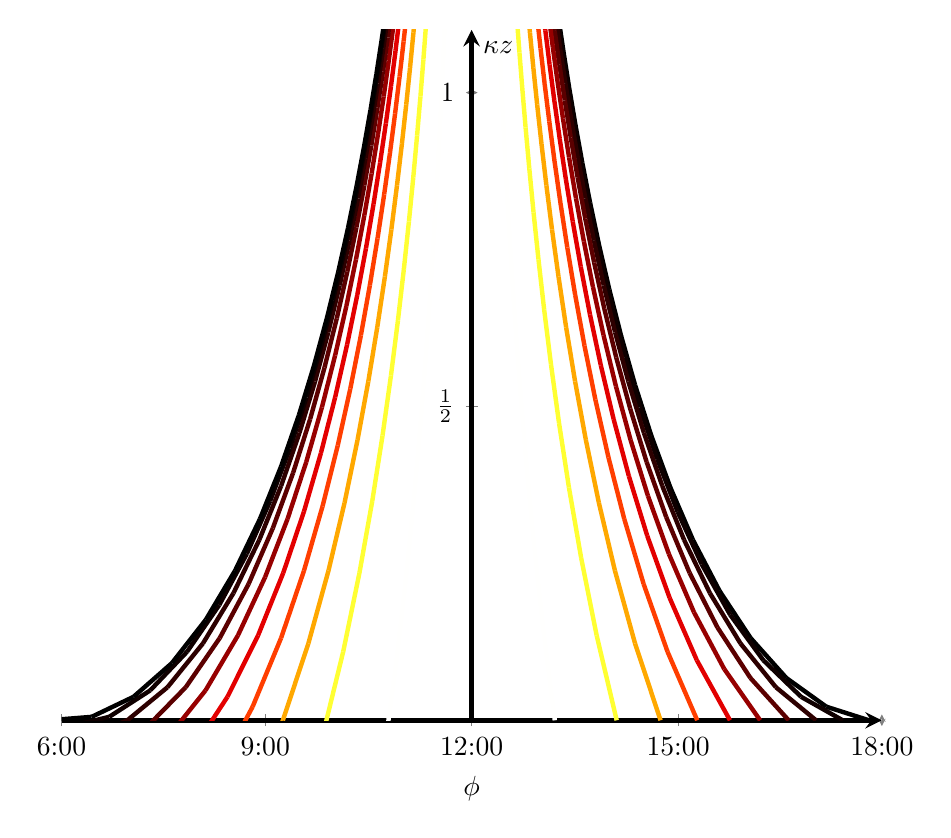
\begin{tikzpicture}[x=1cm,y=1cm]
  \begin{axis}[
      xmin = -1.57,
      xmax = 1.57,
      xlabel = {$\phi$},
      xtick = {-1.57,-0.79,0,0.79,1.57},
      xticklabels = {6:00,9:00,12:00,15:00,18:00},
      axis x line = bottom,
      ymin = 0,
      ymax = 1.1,
      ylabel = {$\kappa z$},
      ytick = {0,0.5,1},
      yticklabels = {$0$,$\tfrac{1}{2}$,$1$},
      axis y line = center,
      colormap/hot2,
      ultra thick,
      every axis/.append style={stealth-stealth}
    ]
    \foreach \w in {-0.95,-0.85,...,0.95}
      \addplot[mesh,domain=0:4,point meta={\w*\w}] (
        {(\w/(abs(\w)))*rad(acos((\w+x)/(sqrt(1+x*x+2*x*\w))))}
      , {0.5*(ln(1+x*x+2*x*\w))} );
  \end{axis};
\end{tikzpicture}
\end{document}
